\documentclass[tikz]{standalone}
\usepackage{xcolor, amsmath, amssymb}
\usetikzlibrary{arrows.meta}
\begin{document}

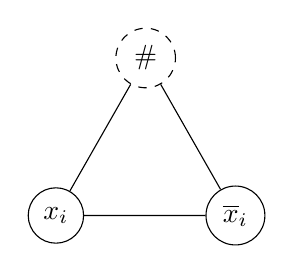
\begin{tikzpicture}[every node/.style={circle,draw},scale=2,minimum size=20pt]
\node[dashed] at(0,0)(r){$\#$};
\node at(-0.57,-1)(t){$x_i$};
\node at(0.57,-1)(f){$\overline x_i$};
\draw(r)--(t)--(f)--(r);
\end{tikzpicture}
 
\end{document}